\documentclass[40pt]{report}
\usepackage{graphicx}
\graphicspath{{Images/}}

\usepackage{amsmath}

\title{\fontsize{30pt}{36pt}\selectfont  FINGERPRINT BASED ATTENDANCE SYSTEM} 
\author{\LARGE Adithya S M\\ \\
S4 : ECE Alpha  \\
\\ \\
\large Department of Electronics and Communication Engineering \\
Rajagiri School of Engineering and Technology \\
\\
\\ \\
\includegraphics[scale=0.5]{logo.jpeg} }


\begin{document}
\maketitle

\begin{abstract}
  To design and implement a figerprint based attendence system using Arduino and figerprint system.The device uses different modules such as arduino,Adafruit optical fingerprint sensor,LCD module.This system would be very promising and as the world is moving closely towards automation and digitization this system can have immense potential to pull of a large market share.
\end{abstract}


\tableofcontents
\listoffigures

\chapter{Introduction}
Fingerprint attendance system is a revolutionary method to modernize the existing roll calls. This devices enables customers and users to go paperfree and decreases the time consumption.  
The device is more feasible and the form factor helps to overcome its present competetors in the market.

 

\begin{figure}[h]
\centering
\includegraphics[scale=0.4]{ss.png}
 
\label{fig_PIC}
\end{figure}

\section{Block Diagram}
\centering
\includegraphics[scale=0.4]{index.jpeg}
\label{sec_Block}
 ~\cite{j_pic}.


\label{fig_Pindia}
\end{figure}
\subsection{Arduino}
\label{sec_arduino}
Arduino is an open-source hardware and software company, project, and user community that designs and manufactures single-board microcontrollers and microcontroller kits for building digital devices.The MCU is a ATMEGA328P based Development board Known for its Versatility and simplicity.
\usepackage{itemize}
\begin{itemize}
\item Microcontroller: ATmega328P.
\item Operating Voltage: 5V.
\item Input Voltage (recommended): 7-12V.
\item Inout Voltage (limit): 6-20V.
\item Digital I/O Pins: 14 (of which 6 provide PWM output)
\item PWM Digital I/O Pins: 6.
\item Analog Input Pins: 6.
\item DC Current per I/O Pin: 20 mA.

\begin{figure}[h]
\centering
\includegraphics[scale=0.4]{arduino.jpeg}

 
\caption{ Arduino}
\end{figure}
\subsection{Adafruit Fingerprint Sensor}

\label{Adafruit FingerPrint Sensor}
\includegraphics[scale=0.4]{fin.jpeg}

 
\caption{FingerPrint Sensor}
\end{figure}
The Adafruit optical fingerprint sensor is a popular sensor compatible with MCU such as Arduino,Raspberry pi etc.The Sensor works in the same range of baud rate as arduino
\usepackage{itemize}
 \begin{itemize}
\item Supply voltage: 3.6 - 6.0VDC.
\item Operating current: 120mA max.
\item Peak current: 150mA max.
\item Fingerprint imaging time: <1.0 seconds.
\item Window area: 14mm x 18mm.
\item Signature file: 256 bytes.
\item Template file: 512 bytes.
\item Storage capacity: 162 templates.
\end{itemize}
\subsection{Liquid Crystal Display}
LCD 16x2 is a 16-pin device that has 2 rows that can accommodate 16 characters each. LCD 16x2 can be used in 4-bit mode or 8-bit mode. It is also possible to create custom characters. It has 8 data lines and 3 control lines that can be used for control purposes.
\usepackage{itemize}
 \begin{itemize}
\item Operating voltage	:5 V
\item Screen resolution	:2-lines x 16 characters
\item Character resolution	:5 x 8 pixels
\item Module dimensions	:80 x 36 x 12 mm
\item Viewing area dimension  :64.5 x 16.4 mm
\end{itemize}

 

 

\section{Arduino Compatible C}
\label{Arduino compatible C}
 The Programming language used here is C which is compatible in c.The Libraries provided simplifies in programs.~\cite{w_knuthwebsite}.


\chapter{Code and expalnation}
\label{ch_SysDesc}
In this system Arduino acts as the main controller.Fingerprint sensor acts an input device and LCD monitor acts a interface to display the actions done to the user.Arduino is development board built on atmega328p.If the System is on mode1:the user can enter their details to the devices as a new entry.if its on second mode the user can check whether their details are fed into the system.Mode 3 enables the user to put down their attendance into the system.Fingerprint sensor transfers the data to the arduino and arduino process the data.

The program is done on Arduino Ide.The project utilises the assistance from different inbuilt libraries they are:
\usepackage{itemize}
 \begin{itemize}
\item #include<EEPROM.h> 
\item #include<LiquidCrystal.h>
\item LiquidCrystal lcd(13,12,11,10,9,8);
\item #include <SoftwareSerial.h>
\item #include <Wire.h>
\item #include "RTClib.h"
 
\item #include "Adafruit_Fingerprint.h"
\end{itemize}
The program works on different modes like accepting new entries,deletion,checking the attendances etc.
all actions are conveyed through the LCD monitor.
 

Sketch uses 283297 bytes (27%) of program storage space. Maximum is 1044464 bytes.
Global variables use 30108 bytes (36%) of dynamic memory, leaving 51812 bytes for local variables. Maximum is 81920 bytes.

\subsection{Code used}

\usepackage{listings}
\begin{lstlisting}[language=python ,frame= single]

#include<EEPROM.h>  
#include<LiquidCrystal.h>  
LiquidCrystal lcd(13,12,11,10,9,8);  
#include <SoftwareSerial.h>  
SoftwareSerial fingerPrint(2, 3);  

#include <Wire.h>  
#include "RTClib.h"  
RTC_DS1307 rtc;  

#include "Adafruit_Fingerprint.h"  
uint8_t id; 
Adafruit_Fingerprint finger = Adafruit_Fingerprint(&fingerPrint);  

#define enroll 14  
#define del 15  
#define up 16  
#define down 17  
#define match 5  
#define indFinger 7  
#define buzzer 5  

#define records 4    

int user1,user2,user3,user4,user5;  

DateTime now;  

void setup()  
{
    delay(1000);  
    lcd.begin(16,2);  
    Serial.begin(9600);  
    pinMode(enroll, INPUT_PULLUP);  
    pinMode(up, INPUT_PULLUP);  
    pinMode(down, INPUT_PULLUP);  
    pinMode(del, INPUT_PULLUP);  
    pinMode(match, INPUT_PULLUP);  
    pinMode(buzzer, OUTPUT);  
    pinMode(indFinger, OUTPUT);  
    digitalWrite(buzzer, LOW);  
    if(digitalRead(enroll) == 0)  
    {  
      digitalWrite(buzzer, HIGH);  
      delay(500);  
      digitalWrite(buzzer, LOW);  
      lcd.clear();  
      lcd.print("Please wait");  
      lcd.setCursor(0,1);  
      lcd.print("Downloding Data");  

      Serial.println("Please wait"); 
      Serial.println("Downloding Data..");  
      Serial.println();  

      Serial.print("S.No.         ");  
      for(int i=0;i<records;i++)  
      { \\
              digitalWrite(buzzer, HIGH);  
      delay(500);    
      digitalWrite(buzzer, LOW);
        Serial.print("         User ID");
        Serial.print(i+1);
        Serial.print("                   ");
      }
      Serial.println();
      int eepIndex=0;
      for(int i=0;i<30;i++)
      {
        if(i+1<10)
        Serial.print('0');
        Serial.print(i+1);
        Serial.print("          ");
        eepIndex=(i*7);
        download(eepIndex);
        eepIndex=(i*7)+210;
        download(eepIndex);
        eepIndex=(i*7)+420;
        download(eepIndex);
        eepIndex=(i*7)+630;
        download(eepIndex);
      //  eepIndex=(i*7)+840;   // 5th user
      //  download(eepIndex);
        Serial.println();
      }
    }
    if(digitalRead(del) == 0)
    {
      lcd.clear();
      lcd.print("Please Wait");
      lcd.setCursor(0,1);
      lcd.print("Reseting.....");
      for(int i=1000;i<1005;i++)
      EEPROM.write(i,0);
      for(int i=0;i<841;i++)
      EEPROM.write(i, 0xff);
      lcd.clear();
      lcd.print("System Reset");
      delay(1000);
    }

    
    lcd.clear();
    lcd.print("   Attendance   ");
    lcd.setCursor(0,1);
    lcd.print("     System     ");
    delay(2000);
    lcd.clear();
    lcd.print("CAM project");
    lcd.setCursor(0,1);
    lcd.print("Adithya S M");
    delay(2000);
          digitalWrite(buzzer, HIGH);
      delay(500);
      digitalWrite(buzzer, LOW);
  for(int i=1000;i<1000+records;i++)
  {
    if(EEPROM.read(i) == 0xff)
        EEPROM.write(i,0);
   }

    finger.begin(57600);
    Serial.begin(9600);
    lcd.clear();
    lcd.print("Finding Module");
    lcd.setCursor(0,1);
    delay(1000);
    if (finger.verifyPassword())
    {
      Serial.println("Found fingerprint sensor!");
      lcd.clear();
      lcd.print("Found Module ");
      delay(1000);
    }
    else
    {
    Serial.println("Did not find fingerprint sensor :(");
    lcd.clear();
    lcd.print("module not Found");
    lcd.setCursor(0,1);
    lcd.print("Check Connections");
    while (1);
    }

     if (! rtc.begin())
       Serial.println("Couldn't find RTC");

    // rtc.adjust(DateTime(F(__DATE__), F(__TIME__)));

    if (! rtc.isrunning())
    {
    Serial.println("RTC is NOT running!");
    // following line sets the RTC to the date & time this sketch was compiled
       rtc.adjust(DateTime(F(__DATE__), F(__TIME__)));
    // This line sets the RTC with an explicit date & time, for example to set
    // January 21, 2014 at 3am you would call:
    // rtc.adjust(DateTime(2014, 1, 21, 3, 0, 0));
    }
lcd.setCursor(0,0);
 lcd.print("Press Match to ");
 lcd.setCursor(0,1);
 lcd.print("Start System");
 delay(2000);

 user1=EEPROM.read(1000);
  user2=EEPROM.read(1001);
   user3=EEPROM.read(1002); 
   user4=EEPROM.read(1003);
    user5=EEPROM.read(1004);
    lcd.clear();
    digitalWrite(indFinger, HIGH);
    
}

void loop()
{
    now = rtc.now();
    lcd.setCursor(0,0);
    lcd.print("Time->");
    lcd.print(now.hour(), DEC);
    lcd.print(':');
    lcd.print(now.minute(), DEC);
    lcd.print(':');
    lcd.print(now.second(), DEC);
    lcd.print("    ");
    lcd.setCursor(0,1);
    lcd.print("Date->");
    lcd.print(now.day(), DEC);
    lcd.print('/');
    lcd.print(now.month(), DEC);
    lcd.print('/');
    lcd.print(now.year(), DEC);
    lcd.print("     ");
    delay(500);
    int result=getFingerprintIDez();
    if(result>0)
    {
              digitalWrite(indFinger, LOW);
              digitalWrite(buzzer, HIGH);
              delay(100);
              digitalWrite(buzzer, LOW);
              lcd.clear();
              lcd.print("ID:");
              lcd.print(result);
              lcd.setCursor(0,1);
              lcd.print("Please Wait....");
              delay(1000);
              attendance(result);
              lcd.clear();
              lcd.print("Attendance ");
              lcd.setCursor(0,1);
              lcd.print("Registed");
              delay(1000);
        digitalWrite(indFinger, HIGH);
        return;
 }
 checkKeys();
 delay(300);
}

//     dmyyhms - 7 bytes
void attendance(int id)
{
  int user=0,eepLoc=0;
  if(id == 1)
  {
    eepLoc=0;
    user=user1++;
  }
  else if(id == 2)
  {
    eepLoc=210;
    user=user2++;
  }
  else if(id == 3)
  {
    eepLoc=420;
    user=user3++;
  }
  else if(id == 4)
  {
    eepLoc=630;
    user=user4++;
  }
  
  else 
  return;
  
    int eepIndex=(user*7)+eepLoc;
    EEPROM.write(eepIndex++, now.hour());
    EEPROM.write(eepIndex++, now.minute());
    EEPROM.write(eepIndex++, now.second());
    EEPROM.write(eepIndex++, now.day());
    EEPROM.write(eepIndex++, now.month());
    EEPROM.write(eepIndex++, now.year()>>8 );
    EEPROM.write(eepIndex++, now.year());

    EEPROM.write(1000,user1);
    EEPROM.write(1001,user2);
    EEPROM.write(1002,user3);
    EEPROM.write(1003,user4);
  //  EEPROM.write(4,user5);   // figth user
}

void checkKeys()
{
   if(digitalRead(enroll) == 0)
   {
    lcd.clear();
    lcd.print("Please Wait");
    delay(1000);
    while(digitalRead(enroll) == 0);
    Enroll();
   }

   else if(digitalRead(del) == 0)
   {
    lcd.clear();
    lcd.print("Please Wait");
    delay(1000);
    delet();
   }
}

void Enroll()
{
   int count=1;
   lcd.clear();
   lcd.print("Enter Finger ID:");

   while(1)
   {
    lcd.setCursor(0,1);
     lcd.print(count);
     if(digitalRead(up) == 0)
     {
       count++;
       if(count>records)
       count=1;
       delay(500);
     }

     else if(digitalRead(down) == 0)
     {
       count--;
       if(count<1)
       count=records;
       delay(500);
     }
     else if(digitalRead(del) == 0)
     {
          id=count;
          getFingerprintEnroll();
          for(int i=0;i<records;i++)
          {
            if(EEPROM.read(i) != 0xff)
            {
              EEPROM.write(i, id);
              break;
            }
          }
          return;
     }

       else if(digitalRead(enroll) == 0)
     {
          return;
     }
 }
}

void delet()
{
   int count=1;
   lcd.clear();
   lcd.print("Enter Finger ID");

   while(1)
   {
    lcd.setCursor(0,1);
     lcd.print(count);
     if(digitalRead(up) == 0)
     {
       count++;
       if(count>records)
       count=1;
       delay(500);
     }

     else if(digitalRead(down) == 0)
     {
       count--;
       if(count<1)
       count=records;
       delay(500);
     }
     else if(digitalRead(del) == 0)
     {
          id=count;
          deleteFingerprint(id);
          for(int i=0;i<records;i++)
          {
            if(EEPROM.read(i) == id)
            {
              EEPROM.write(i, 0xff);
              break;
            }
          }
          return;
     }

       else if(digitalRead(enroll) == 0)
     {
          return;
     }
 }
}

uint8_t getFingerprintEnroll()
{
  int p = -1;
  lcd.clear();
  lcd.print("finger ID:");
  lcd.print(id);
  lcd.setCursor(0,1);
  lcd.print("Place Finger");
  delay(2000);
  while (p != FINGERPRINT_OK)
  {
    p = finger.getImage();
    switch (p)
    {
    case FINGERPRINT_OK:
      Serial.println("Image taken");
      lcd.clear();
      lcd.print("Image taken");
      break;
    case FINGERPRINT_NOFINGER:
      Serial.println("No Finger");
      lcd.clear();
      lcd.print("No Finger");
      break;
    case FINGERPRINT_PACKETRECIEVEERR:
      Serial.println("Communication error");
      lcd.clear();
      lcd.print("Comm Error");
      break;
    case FINGERPRINT_IMAGEFAIL:
      Serial.println("Imaging error");
      lcd.clear();
      lcd.print("Imaging Error");
      break;
    default:
      Serial.println("Unknown error");
       lcd.clear();
      lcd.print("Unknown Error");
      break;
    }
  }

  // OK success!

  p = finger.image2Tz(1);
  switch (p) {
    case FINGERPRINT_OK:
      Serial.println("Image converted");
      lcd.clear();
      lcd.print("Image converted");
      break;
    case FINGERPRINT_IMAGEMESS:
      Serial.println("Image too messy");
       lcd.clear();
       lcd.print("Image too messy");
      return p;
    case FINGERPRINT_PACKETRECIEVEERR:
      Serial.println("Communication error");
            lcd.clear();
      lcd.print("Comm Error");
      return p;
    case FINGERPRINT_FEATUREFAIL:
      Serial.println("Could not find fingerprint features");
            lcd.clear();
      lcd.print("Feature Not Found");
      return p;
    case FINGERPRINT_INVALIDIMAGE:
      Serial.println("Could not find fingerprint features");
                  lcd.clear();
      lcd.print("Feature Not Found");
      return p;
    default:
      Serial.println("Unknown error");
                  lcd.clear();
      lcd.print("Unknown Error");
      return p;
  }

  Serial.println("Remove finger");
  lcd.clear();
  lcd.print("Remove Finger");
  delay(2000);
  p = 0;
  while (p != FINGERPRINT_NOFINGER) {
    p = finger.getImage();
  }
  Serial.print("ID "); Serial.println(id);
  p = -1;
  Serial.println("Place same finger again");
   lcd.clear();
      lcd.print("Place Finger");
      lcd.setCursor(0,1);
      lcd.print("   Again");
  while (p != FINGERPRINT_OK) {
    p = finger.getImage();
    switch (p) {
    case FINGERPRINT_OK:
      Serial.println("Image taken");
      break;
    case FINGERPRINT_NOFINGER:
      Serial.print(".");
      break;
    case FINGERPRINT_PACKETRECIEVEERR:
      Serial.println("Communication error");
      break;
    case FINGERPRINT_IMAGEFAIL:
      Serial.println("Imaging error");
      break;
    default:
      Serial.println("Unknown error");
      return 0;
    }
  }

  // OK success!

  p = finger.image2Tz(2);
  switch (p) {
    case FINGERPRINT_OK:
      Serial.println("Image converted");
      break;
    case FINGERPRINT_IMAGEMESS:
      Serial.println("Image too messy");
      return p;
    case FINGERPRINT_PACKETRECIEVEERR:
      Serial.println("Communication error");
      return p;
    case FINGERPRINT_FEATUREFAIL:
      Serial.println("Could not find fingerprint features");
      return p;
    case FINGERPRINT_INVALIDIMAGE:
      Serial.println("Could not find fingerprint features");
      return p;
    default:
      Serial.println("Unknown error");
      return p;
  }

  // OK converted!
  Serial.print("Creating model for #");  Serial.println(id);

  p = finger.createModel();
  if (p == FINGERPRINT_OK) {
    Serial.println("Prints matched!");
  } else if (p == FINGERPRINT_PACKETRECIEVEERR) {
    Serial.println("Communication error");
    return p;
  } else if (p == FINGERPRINT_ENROLLMISMATCH) {
    Serial.println("Fingerprints did not match");
    return p;
  } else {
    Serial.println("Unknown error");
    return p;
  }

  Serial.print("ID "); Serial.println(id);
  p = finger.storeModel(id);
  if (p == FINGERPRINT_OK) {
    Serial.println("Stored!");
    lcd.clear();
    lcd.print("Stored!");
    delay(2000);
  } else if (p == FINGERPRINT_PACKETRECIEVEERR) {
    Serial.println("Communication error");
    return p;
  } else if (p == FINGERPRINT_BADLOCATION) {
    Serial.println("Could not store in that location");
    return p;
  } else if (p == FINGERPRINT_FLASHERR) {
    Serial.println("Error writing to flash");
    return p;
  }
  else {
    Serial.println("Unknown error");
    return p;
  }
}

int getFingerprintIDez()
{
  uint8_t p = finger.getImage();

  if (p != FINGERPRINT_OK)
  return -1;

  p = finger.image2Tz();
  if (p != FINGERPRINT_OK)
  return -1;

  p = finger.fingerFastSearch();
  if (p != FINGERPRINT_OK)
  {
   lcd.clear();
   lcd.print("Finger Not Found");
   lcd.setCursor(0,1);
   lcd.print("Try Later");
   delay(2000);
  return -1;
  }
  // found a match!
  Serial.print("Found ID #");
  Serial.print(finger.fingerID);
  return finger.fingerID;
}

uint8_t deleteFingerprint(uint8_t id)
{
  uint8_t p = -1;
  lcd.clear();
  lcd.print("Please wait");
  p = finger.deleteModel(id);
  if (p == FINGERPRINT_OK)
  {
    Serial.println("Deleted!");
    lcd.clear();
    lcd.print("Figer Deleted");
    lcd.setCursor(0,1);
    lcd.print("Successfully");
    delay(1000);
  }

  else
  {
    Serial.print("Something Wrong");
    lcd.clear();
    lcd.print("Something Wrong");
    lcd.setCursor(0,1);
    lcd.print("Try Again Later");
    delay(2000);
    return p;
  }
}

void download(int eepIndex)
{
            
            if(EEPROM.read(eepIndex) != 0xff)
            {
              Serial.print("T->");
              if(EEPROM.read(eepIndex)<10)
              Serial.print('0');
              Serial.print(EEPROM.read(eepIndex++));
              Serial.print(':');  
              if(EEPROM.read(eepIndex)<10)
              Serial.print('0');
              Serial.print(EEPROM.read(eepIndex++));
              Serial.print(':'); 
              if(EEPROM.read(eepIndex)<10)
              Serial.print('0');
              Serial.print(EEPROM.read(eepIndex++));
              Serial.print("   D->");
              if(EEPROM.read(eepIndex)<10)
              Serial.print('0');
              Serial.print(EEPROM.read(eepIndex++));
              Serial.print('/');
              if(EEPROM.read(eepIndex)<10)
              Serial.print('0');           
              Serial.print(EEPROM.read(eepIndex++));
              Serial.print('/');            
              Serial.print(EEPROM.read(eepIndex++)<<8 | EEPROM.read(eepIndex++));
            }
            else
            {
               Serial.print("---------------------------");
            }

            Serial.print("         ");
}


 
\end{lstlisting}

\subsection{Simulation output}
 
\begin{figure}[h]
\centering
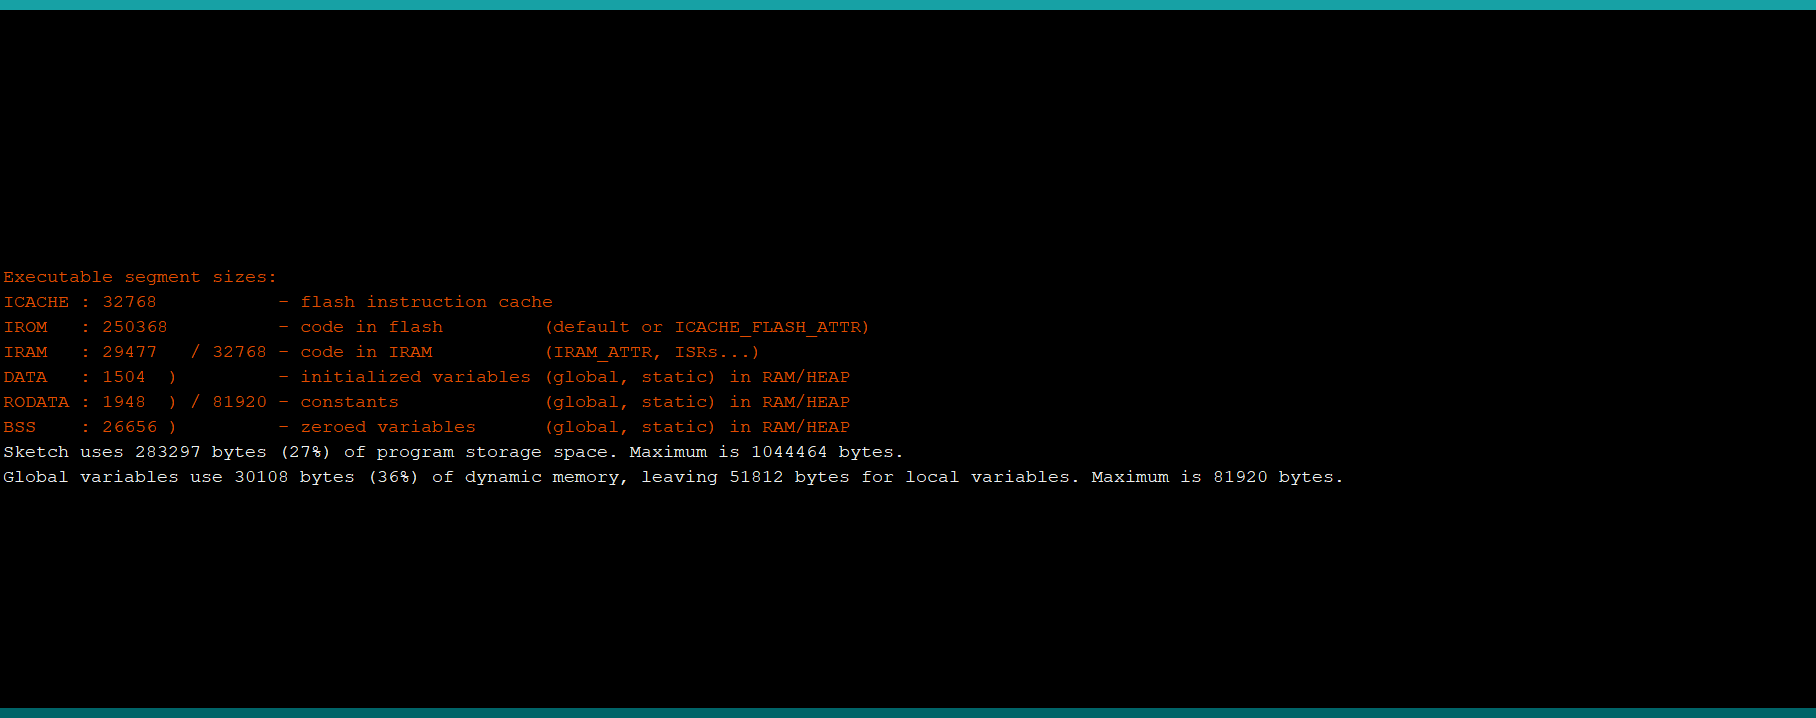
\includegraphics[scale=0.4]{fg.png}
 
\label{Simulation output}
\end{figure}
\subsection{Conclussion}
\label{conc}
The assigned problem statement has been simulated and verified using arduino.

\begin{thebibliography}{10}
 

\bibitem{j_pic}https://learn.adafruit.com/adafruit-optical-fingerprint-sensor

\bibitem{w_knuthwebsite}
https://whatis.techtarget.com/definition/LCD-liquid-crystal-display#:~:text=LCD%20(Liquid%20Crystal%20Display)%20is,its%20primary%20form%20of%20operation.&text=As%20LCDs%20have%20replaced%20older,display%20technologies%20such%20as%20OLEDs.

\bibitem{w_knuthwebsite}
 https://www.arduino.cc/reference/en/libraries/adafruit-fingerprint-sensor-library/

\end{thebibliography}

\end{document}

